\documentclass[11pt,a4paper]{article}
\usepackage[margin=18mm,headheight=24pt]{geometry}
\usepackage[T1]{fontenc}
\usepackage[english]{babel}
\usepackage{lmodern}
\usepackage{microtype}
\usepackage{amsmath,amssymb}
\usepackage{siunitx}
\usepackage{tikz}
\usetikzlibrary{arrows.meta,calc,angles,quotes}
\usepackage{enumitem}
\usepackage{xcolor}
\usepackage{fancyhdr}
\usepackage{lastpage}
\usepackage[hidelinks]{hyperref}

\definecolor{VectorGreen}{HTML}{174A38}
\definecolor{VectorAccent}{HTML}{216343}
\definecolor{VectorMint}{HTML}{E2F0E5}
\definecolor{VectorCoral}{HTML}{C45136}
\definecolor{VectorInk}{HTML}{203B31}
\definecolor{VectorMuted}{HTML}{5F7468}

\color{VectorInk}
\setlength{\parindent}{0pt}
\setlength{\parskip}{0.55em}
\setlist[enumerate]{leftmargin=*,itemsep=0.45em,topsep=0.35em}
\sisetup{per-mode=symbol}

\pagestyle{fancy}
\fancyhf{}
\lhead{\textcolor{VectorMuted}{Vectors · Exercise session}}
\rhead{\textcolor{VectorMuted}{Addition and subtraction}}
\cfoot{\textcolor{VectorMuted}{\thepage\ / \pageref*{LastPage}}}
\renewcommand{\headrulewidth}{0.4pt}
\renewcommand{\headrule}{\hbox to\headwidth{\color{VectorMint}\leaders\hrule height \headrulewidth\hfill}}

\newcommand{\sessiontitle}[2]{%
  {\color{VectorGreen}\fontsize{25}{29}\selectfont\bfseries #1\par}
  \vspace{0.2em}
  {\color{VectorMuted}\large #2\par}
  \vspace{0.55em}
  {\color{VectorAccent}\rule{\textwidth}{1.5pt}}
}

\newcommand{\problemheading}[2]{%
  {\color{VectorAccent}\small\bfseries\MakeUppercase{Problem #1}}\par
  {\color{VectorGreen}\LARGE\bfseries #2}\par
  \vspace{0.25em}
}

\newcommand{\prediction}[1]{%
  \begin{center}
  \colorbox{VectorMint}{\parbox{0.92\linewidth}{\textbf{Predict before calculating.} #1}}
  \end{center}
}

\newcommand{\checkpoint}[1]{%
  \begin{center}
  \fcolorbox{VectorAccent}{white}{\parbox{0.91\linewidth}{\textbf{Reasoning checkpoint.} #1}}
  \end{center}
}

\newcommand{\worklines}[1]{%
  \par\vspace{0.25em}
  {\color{VectorMuted}\small\textit{Working and explanation}}\par
  \foreach \n in {1,...,#1}{\vspace{0.54cm}\noindent\textcolor{VectorMint}{\rule{\linewidth}{0.35pt}}\par}
}

\newcommand{\answerbox}[1]{%
  \begin{center}
  \colorbox{VectorMint}{\parbox{0.92\linewidth}{\textbf{Answer.} #1}}
  \end{center}
}


\begin{document}

\sessiontitle{Solutions: Vectors that fool intuition}{Instructor copy · Vector addition and subtraction}

\problemheading{1}{How can $600+600=600$?}  

Let each force make an angle $\theta$ with east. Symmetry makes the vertical components cancel. The horizontal components add:
\[ 
  600\cos\theta+600\cos\theta=600. 
\]
Therefore $2\cos\theta=1$, so $\theta=60^\circ$. The two ropes lie $60^\circ$ above and below east, giving an angle of
\[
  \boxed{120^\circ\text{ between the ropes}.} 
\]

\begin{center}
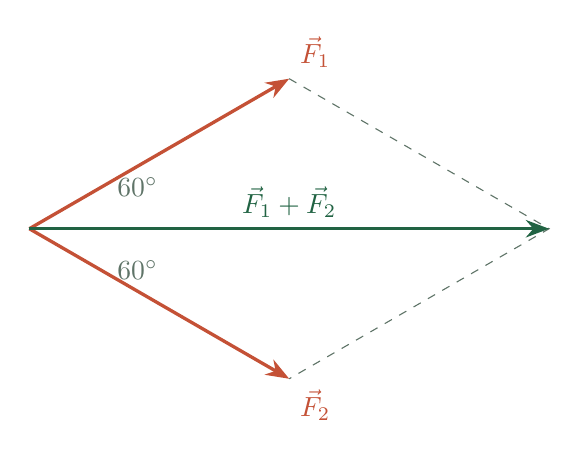
\begin{tikzpicture}[>=Stealth,scale=1.1]
  \coordinate (O) at (0,0);
  \coordinate (A) at (3,1.732);
  \coordinate (B) at (3,-1.732);
  \coordinate (C) at (6,0);
  \draw[->,very thick,VectorCoral] (O)--(A) node[above right] {$\vec F_1$};
  \draw[->,very thick,VectorCoral] (O)--(B) node[below right] {$\vec F_2$};
  \draw[dashed,VectorMuted] (A)--(C)--(B);
  \draw[->,very thick,VectorAccent] (O)--(C) node[midway,above] {$\vec F_1+\vec F_2$};
  \node[VectorMuted] at (1.25,0.48) {$60^\circ$};
  \node[VectorMuted] at (1.25,-0.48) {$60^\circ$};
\end{tikzpicture}
\end{center}

For two \SI{600}{N} pulls, the resultant can range from $0$ to \SI{1200}{N}. It is zero when the forces are opposite and \SI{1200}{N} when they point together.

\answerbox{Vector addition combines components and directions. Only parallel vectors pointing the same way allow their magnitudes to be added directly.}

\checkpoint{Ask students why an obtuse angle is already plausible before calculation: substantial sideways cancellation is needed for the sum to be no larger than one pull.}

\vfill

\clearpage
\problemheading{2}{Same sum. Same journey?}

Both finish at $(3,4)$ m after \SI{7}{s}. Hence both have
\[
\Delta\vec r=(3,4)\ \si{m},\quad |\Delta\vec r|=\SI{5}{m},\quad
\vec v_{\rm avg}=\left(\frac37,\frac47\right)\ \si{m/s}.
\]
Each walks \SI{7}{m}, so each average speed is \SI{1}{m/s}. The magnitude of each average velocity is only $5/7\ \si{m/s}$.

For Aruzhan,
\[
\vec r_A(t)=
\begin{cases}
(t,0),&0\le t\le3,\\
(3,t-3),&3\le t\le7.
\end{cases}
\]
For Daniyar,
\[
\vec r_D(t)=
\begin{cases}
(0,t),&0\le t\le4,\\
(t-4,4),&4\le t\le7.
\end{cases}
\]
These positions are equal only at $t=0$ and $t=7$ s. Apart from the common start, they meet only at the finish.

At $t=3.5$ s,
\[
\vec r_A=(3,0.5)\ \si{m},\qquad \vec r_D=(0,3.5)\ \si{m},
\]
so the vector from Aruzhan to Daniyar is
\[
\vec r_D-\vec r_A=\boxed{(-3,3)\ \si{m}}.
\]

\answerbox{$\vec a+\vec b=\vec b+\vec a$ guarantees the same resultant displacement and endpoint. It does not guarantee the same path or the same position at intermediate times.}

\clearpage
\problemheading{3}{Two apps disagree—or do they?}

App E uses the basis vectors east and north:
\[
\vec d=3\,\hat e_{\rm east}+4\,\hat e_{\rm north}.
\]
App N calls north its first positive direction and west its second. Therefore
\[
\vec d=4\,\hat e_{\rm north}-3\,\hat e_{\rm west}.
\]
The minus sign means \SI{3}{km} opposite west, which is east. Converting App N's report to east--north coordinates gives
\[
(4,-3)_{(\rm north,west)}=(3,4)_{(\rm east,north)}.
\]

The calculation $(3,4)+(4,-3)$ combines coordinate entries attached to different basis directions. The first entries do not even refer to the same physical axis: one is east and the other is north.

Because the two reports describe the same physical displacement, their difference must be zero. After conversion,
\[
(3,4)_{E}-(3,4)_{E}=\boxed{(0,0)}.
\]

\answerbox{Before adding or subtracting component pairs, express every vector in the same coordinate system, with the same axes, positive directions, and units.}

\checkpoint{Changing axes changes the component numbers. It does not rotate the actual displacement or create a second displacement.}

\vfill

\clearpage
\problemheading{4}{Equal speeds on a collision course}

B's position relative to A is
\[
\vec r_{B/A}(0)=\vec r_B-\vec r_A=(8,-8)\ \si{m}.
\]
B's velocity relative to A is
\[
\vec v_{B/A}=\vec v_B-\vec v_A=(0,4)-(4,0)=(-4,4)\ \si{m/s}.
\]
Thus
\[
\vec r_{B/A}(t)=(8,-8)+t(-4,4).
\]
For a collision, both components must be zero at the same time:
\[
8-4t=0,\qquad -8+4t=0.
\]
Both give $t=\SI{2}{s}$. The meeting position is
\[
\vec r_A(2)=(0,0)+(4,0)(2)=\boxed{(8,0)\ \si{m}}.
\]
Checking with B gives $(8,-8)+(0,4)(2)=(8,0)$ m.

\begin{center}
\begin{tikzpicture}[>=Stealth,scale=0.72]
  \draw[->,VectorMuted] (-0.4,0)--(10.6,0) node[right] {east};
  \draw[->,VectorMuted] (0,-8.7)--(0,2.2) node[above] {north};
  \draw[very thick,VectorAccent,->] (0,0)--(8,0);
  \draw[very thick,VectorCoral,->] (8,-8)--(8,0);
  \fill[VectorGreen] (8,0) circle (4pt) node[above right] {$t=\SI{2}{s}$};
  \draw[->,very thick,VectorGreen] (8,-8)--(4,-4) node[midway,above left] {$\vec v_{B/A}$};
\end{tikzpicture}
\end{center}

\answerbox{Equal speed means equal velocity magnitudes. It says nothing about whether the relative velocity points along the line that closes the relative-position vector.}

\checkpoint{The compact collision test is whether one positive time makes $\vec r_{B/A}(0)+\vec v_{B/A}t=\vec 0$.}

\end{document}

